\section{Library Configuration}
\label{ssec:config}

The requirements of PVSLM are:
curl
PVS

Every package must have a dependencies file, where the relations between its theories and other packages are specified. The file has to be named ``top.dep'' and be located within the package in a folder named ``pvsbin''. 

The syntax for the dependencies file is described below on Table \ref{tab:bnf}.

\begin{table}[h!]
  \begin{center}
    BNF: Dependencies syntax PVS Library \\
    \begin{tabular}{ l l p{8cm} }

       \hline
      $<$part\_one$>$ & ::= & ``/'' $<$theories\_list$>$\\
      $<$theories\_list$>$ & ::= &  $<$theory$>$ $|$ $<$theory$>$ ``,'' $<$theories\_list$>$\\
      \\
      $<$part\_two$>$ & ::= &  $<$package\_dep$>$ ``/'' $<$theories\_dep$>$\\
      $<$theories\_dep$>$ & ::= &  $<$theory\_dep$>$ $|$ $<$theory\_dep$>$ ``,'' $<$theories\_dep$>$\\
      \\
      $<$part\_three$>$ & ::= &  $<$theory$>$ ``:'' $<$dependencies\_pkg$>$\\
      $<$dependencies\_pkg$>$ & ::= &  $<$package\_dep$>$ ``@'' $<$theory\_dep$>$ $|$ $<$package\_dep$>$ ``@'' $<$theory\_dep$>$ ``,'' $<$dependencies\_pkg$>$\\
      \hline
    \end{tabular}
  \end{center}
  \label{tab:bnf}
\end{table}

There are three parts in the syntax. The first one lists the theories of the package, this line must begin with a backslash `\textbackslash' followed by the theories separated by commas. The second part is the list of the package and theories with which there are dependency relations, one package per line. Each line begins with the package name, then a backslash `\textbackslash' and the theories separated by commas. This is the most important section of the file for PVSLM, because of its meaning. 

Finally there is the list of relations between the theories, no matter what package are them from. Each line begins with the name of the theory followed by colon `:' and the list of theories with which there is relation, if the the theory is from another package it is necessary to include the name of the package followed by the symbol `@' before the name of the theory, otherwise the name of the theory is enough.

\begin{figure}[h!]
  \centering
  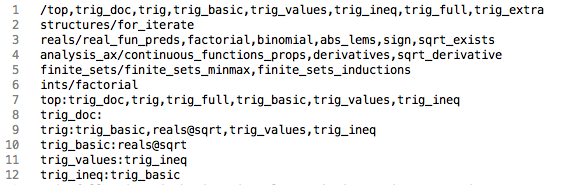
\includegraphics[scale=0.6]{syntax}
  \caption{Dependencies file syntax example}
  \label{fig:syntax}
\end{figure}

In the Figure \ref{fig:syntax} there are examples for each of the cases explained above. The example is taken from a file of nasalib.
